\documentclass[review]{elsarticle}
 \usepackage{fullpage}
 \usepackage{amsfonts} 
 \usepackage{amsmath}
 \usepackage{amsthm}
% \usepackage{amsrefs}
% \def\bibsection{\section*{References}}
 \usepackage{pifont}
 \usepackage{natbib}
 \usepackage{geometry}
 \usepackage{graphicx}
 \usepackage{hyperref}
 
%ming's package for numerical section 
\RequirePackage{lineno}
\usepackage{subfig}
\usepackage{amssymb}
\usepackage{multirow}
\usepackage{subfig}
\usepackage{setspace}
\usepackage{url}
\usepackage{color}

%environment
\newtheorem{thm}{Theorem}
\newtheorem{lem}[thm]{Lemma}
\newtheorem{cor}{Corollary}
\newdefinition{rmk}{Remark}
\newtheorem*{defi*}{Definition}
%\newproof{proof}{Proof}
\begin{document}

\begin{frontmatter}
\title{Ranking Distance Correlation}
%\author[jhuams]{CS, JV, YP, CEP, etc?}

\end{frontmatter}

\section{Set-up}
Let $X \sim U(0,1)^{d} \in \mathbb{R}^{d}$, where $U$ is the uniform distribution, $d$ is the dimension size. 

Let $Y=f(X) * A \in \mathbb{R}$, where $f: \mathbb{R}^{d} \rightarrow \mathbb{R}^{d}$ is certain function of $X$, and $A$ is a $d \times 1$ vector. So $Y$ is a one-dimensional variable that is related to $X$.

For the choice of $f()$, we use linear, quadratic, cubic, sine period $1/2$, sine period $1/8$, $X^{0.25}$, circle, step function, exponential, and log function. Please see the code for detail. 

For the choice of $A$, we use $A(i)=1/i, \forall i=1,\ldots,d$, so that the entries of $A$ decays as the dimension increases. 

For another choice of $A$, we use $A(i)=1/ \left\lceil d * C(i) \right\rceil$, where $C_{i} \stackrel{i.i.d.}{\sim} U(0,1)$. So $A$ randomly decays as the dimension increases, rather than fixed decay in the previous case. In experiment, $A$ is pre-generated and never changed in each Monte-Carlo run.

\section{Independence tests}
Given two sample data $\mathcal{X}$ and $\mathcal{Y}$ of size $n \times d$ and size $n \times 1$ ($n$ is the sample size), the null hypothesis is that they are not independent. The alternative hypothesis is they are independent.

Fix $f$ and $A$. To test whether Ranking Distance Correlation improves over distance correlation, the experiment is done as follows: we first obtain $\mathcal{X}$ and $\mathcal{Y}$ by generate $(X,Y)$ for $n=100$ pairs, and calculate the distance correlation and Ranking Distance Correlation between them. Repeat it for $500$ Monte-Carlo replicates, we obtain the empirical distribution of DC and RDC for that type of $f$ and $A$, which are the test statistics under the null.

Now repeat the same procedure, but $\mathcal{X}$ and $\mathcal{Y}$ are generated from $(Z,Y)$ for $n=100$ pairs. $Z \sim U(0,1)^{d} \in \mathbb{R}^{d}$ but is independent from $X$, so $Z$ is also independent from $Y$. After $500$ Monte-Carlo replicates, we obtain the empirical distribution of DC and RDC under the alternative.

Given DC and RDC under the null and the alternative, we calculate the testing power at type $1$ error level $0.95$. To assess the effect for high-dimensional data, we do the experiment for $d=1,\ldots,1000$ at $n=100$. 

The next two sections show the results. It is clear that no matter in fixed decay or random decay, RDC performs at least similarly as DC; and for more than half the function types, RDC is significantly better than DC as the dimension increases. This shows that RDC has a very obvious advantage in identifying correlation among high-dimensional data.

The last section considers $Y=f(X*A)$ with fixed decay, which also shows the advantage of RDC.

\section{$y=f(x)*A$ with fixed decay}

\begin{figure}[htbp]
\subfloat[]{
\includegraphics[width=0.5\textwidth]{data/hd1/TibsSimuIndDimType1N100}
}
\hfil
\subfloat[]{
\includegraphics[width=0.5\textwidth]{data/hd1/TibsSimuIndDimType2N100}
}
\hfil
\subfloat[]{
\includegraphics[width=0.5\textwidth]{data/hd1/TibsSimuIndDimType3N100}
}
\hfil
\subfloat[]{
\includegraphics[width=0.5\textwidth]{data/hd1/TibsSimuIndDimType4N100}
}
\hfil
\subfloat[]{
\includegraphics[width=0.5\textwidth]{data/hd1/TibsSimuIndDimType5N100}
}
\hfil
\subfloat[]{
\includegraphics[width=0.5\textwidth]{data/hd1/TibsSimuIndDimType6N100}
}
\caption{Fixed Decay 1}
\label{}
\end{figure}

\begin{figure}[htbp]
\subfloat[]{
\includegraphics[width=0.5\textwidth]{data/hd1/TibsSimuIndDimType7N100}
}
\hfil
\subfloat[]{
\includegraphics[width=0.5\textwidth]{data/hd1/TibsSimuIndDimType8N100}
}
\hfil
\subfloat[]{
\includegraphics[width=0.5\textwidth]{data/hd1/TibsSimuIndDimType9N100}
}
\hfil
\subfloat[]{
\includegraphics[width=0.5\textwidth]{data/hd1/TibsSimuIndDimType10N100}
}
\caption{Fixed Decay 2}
\label{}
\end{figure}

\section{$y=f(x)*A$ with random decay}

\begin{figure}[htbp]
\subfloat[]{
\includegraphics[width=0.5\textwidth]{data/hd2/TibsSimuIndDimType1N100}
}
\hfil
\subfloat[]{
\includegraphics[width=0.5\textwidth]{data/hd2/TibsSimuIndDimType2N100}
}
\hfil
\subfloat[]{
\includegraphics[width=0.5\textwidth]{data/hd2/TibsSimuIndDimType3N100}
}
\hfil
\subfloat[]{
\includegraphics[width=0.5\textwidth]{data/hd2/TibsSimuIndDimType4N100}
}
\hfil
\subfloat[]{
\includegraphics[width=0.5\textwidth]{data/hd2/TibsSimuIndDimType5N100}
}
\hfil
\subfloat[]{
\includegraphics[width=0.5\textwidth]{data/hd2/TibsSimuIndDimType6N100}
}
\caption{Random Decay 1}
\label{}
\end{figure}

\begin{figure}[htbp]
\subfloat[]{
\includegraphics[width=0.5\textwidth]{data/hd2/TibsSimuIndDimType7N100}
}
\hfil
\subfloat[]{
\includegraphics[width=0.5\textwidth]{data/hd2/TibsSimuIndDimType8N100}
}
\hfil
\subfloat[]{
\includegraphics[width=0.5\textwidth]{data/hd2/TibsSimuIndDimType9N100}
}
\hfil
\subfloat[]{
\includegraphics[width=0.5\textwidth]{data/hd2/TibsSimuIndDimType10N100}
}
\caption{Random Decay 2}
\label{}
\end{figure}

\section{$Y=f(X*A)$ with fixed decay}
\begin{figure}[htbp]
\subfloat[]{
\includegraphics[width=0.5\textwidth]{data/hd3/TibsSimuIndDimType1N100}
}
\hfil
\subfloat[]{
\includegraphics[width=0.5\textwidth]{data/hd3/TibsSimuIndDimType2N100}
}
\hfil
\subfloat[]{
\includegraphics[width=0.5\textwidth]{data/hd3/TibsSimuIndDimType3N100}
}
\hfil
\subfloat[]{
\includegraphics[width=0.5\textwidth]{data/hd3/TibsSimuIndDimType4N100}
}
\hfil
\subfloat[]{
\includegraphics[width=0.5\textwidth]{data/hd3/TibsSimuIndDimType5N100}
}
\hfil
\subfloat[]{
\includegraphics[width=0.5\textwidth]{data/hd3/TibsSimuIndDimType6N100}
}
\caption{Fix Decay 3}
\label{}
\end{figure}

\begin{figure}[htbp]
\subfloat[]{
\includegraphics[width=0.5\textwidth]{data/hd3/TibsSimuIndDimType8N100}
}
\hfil
\subfloat[]{
\includegraphics[width=0.5\textwidth]{data/hd3/TibsSimuIndDimType9N100}
}
\hfil
\subfloat[]{
\includegraphics[width=0.5\textwidth]{data/hd3/TibsSimuIndDimType10N100}
}
\caption{Fix Decay 4}
\label{}
\end{figure}


%\bibliographystyle{ieeetr}
%\bibliography{references}

\end{document}